\documentclass[12pt,a4paper]{beamer}
\usetheme{Amsterdam}
%\usecolortheme{beaver}
\usepackage[english,french]{babel}
%\usepackage[utf8]{inputenc}  
\usepackage[T1]{fontenc}
\usepackage{fontspec}
\usepackage{amsmath}
\usepackage{amsfonts}
\usepackage{amssymb}
\usepackage{tikz}
\usepackage{listings}
\usepackage{pgfplots}
%\pgfplotsset{compat=1.14}
\pgfplotsset{compat=newest}
\usepackage{color}
\usepackage{marvosym}

%Underline in color
\newcommand{\coloruline}[3]{\emph{\textcolor{#1}{\underline{#2\textcolor{black}{#3}}}}}



\lstset{
  language=Java,
  commentstyle=\color{mygreen},    % comment style
  stringstyle=\color{mymauve},     % string literal style
  keywordstyle=\color{blue},       % keyword style
  basicstyle=\footnotesize        % the size of the fonts that are used for the code
}

\title{\textbf{Algorithmique avancée}}
\subtitle{Tables de hachage}
\author{Frédéric Guyomarch}
\date{2018/2019 - Semestre 3}
\institute % (optional)
{

  Université de Lille1\\
  IUT-A de Lille

}
 

 
\logo{
\includegraphics[width=5em]{figs/iutaustl}}

%Remove Figure prefix on captures
\setbeamertemplate{caption}{\raggedright\insertcaption\par}

%Remove Control bar
\beamertemplatenavigationsymbolsempty

\setbeamertemplate{blocks}[rounded]
\newcommand{\hl}[1]{\textcolor{blueemph}{#1}}


\definecolor{mygreen}{rgb}{0,0.6,0}
\definecolor{mygray}{rgb}{0.5,0.5,0.5}
\definecolor{mymauve}{rgb}{0.58,0,0.82}
\definecolor{greenfluo}{rgb}{0,255,0}
\definecolor{blueemph}{RGB}{17,59,94}


\begin{document}

\begin{frame}
\titlepage
\end{frame}

\begin{frame}{Introduction}{Table de hachage}

Une table de hachage correspond à un ensemble de valeurs identifiées par des clés et spécifie plusieurs opérations : 
\begin{itemize}
\item \texttt{recherche(K key)}: retourne l'élément de clé key
\item \texttt{insert(K key, V val)}: (écrit par-dessus si key existe) 
\item \texttt{supprime(K key)}
\end{itemize}
C'est une implémentation d'un type de données abstrait Dictionnaire (associations clé et valeurs).
\end{frame}


\begin{frame}{Introduction}{Table de hachage en résumé}

\begin{itemize}
\item Une structure de type dictionnaire
\item Contenant des couples (clé,valeur)
\item La clé identifie la valeur 
\item Pas de notion notion d'ordre
\item Pas de doublon
\item Basée sur les tableaux
\end{itemize}
\pause 
 \hl{\textbf{\Smiley Insertion et recherche en temps quasi constant!}}
\end{frame}


\begin{frame}{Motivations}{}

\begin{itemize}
\item Un dictionnaire
\item Base de données
\item Historiquement pour les compilateurs (table des symboles)
\item Vérification de mots de passe
\item Maintenir une liste noire d'adresses ip
\end{itemize}

\end{frame}

\begin{frame}[t]{Application}{Déduplication}
\underline{Entrée} : Un flux d'objets\\
\underline{But} : Enlever les doublons (ne garder que des objets uniques)\\
Exemple: Repérer des visiteurs uniques sur une site web
\end{frame}


\begin{frame}[t]{Application}{Problème de 2-Sum}
\underline{Entrée} : Un tableau d'entiers non trié $T$, une valeur cible $z$.\\
\underline{But} : Déterminer s'il existe deux entiers $x$ et $y$ dans $T$ tel que $x + y = z$.
\end{frame}



\begin{frame}
\tableofcontents
\end{frame}

\section{Introduction au hachage}


\begin{frame}{Table de hachage : Principe général}
\centering \textbf{Des couples (clé,valeur) stockés dans un tableau}
\begin{block}{}
\begin{figure}
\includegraphics[scale=0.3]{figs/ht_global}
\end{figure}
\end{block}
\pause
$\Rightarrow$ une association clé du couple/indice du tableau.
\end{frame}

\begin{frame}{Table de hachage : Principe général}

\begin{block}{Problématique}
Comment ranger les éléments dans le tableau de manière à avoir une recherche en accès direct?
\end{block}
\pause
\begin{itemize}
\item Facile a priori si ma clé est un indice (idem tableau) 
\end{itemize}


\end{frame}

\begin{frame}{Exemple}
Exemple: Un registre d'employés 

\only<1>{
\begin{figure}
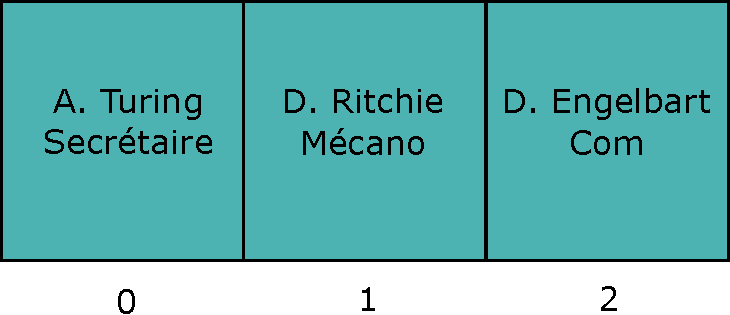
\includegraphics[scale=0.45]{figs/ht_employ}
\end{figure}}



\only<2->{
\begin{figure}
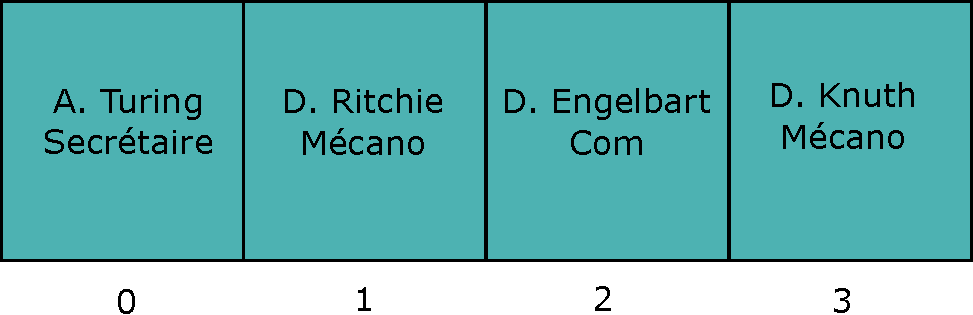
\includegraphics[scale=0.45]{figs/ht_employ2}
\end{figure}
A chaque embauche, on incrémente la clé.

}
\only<3->{
\begin{itemize}
\item La clé correspond à l'indice
\item Les clés sont en séquences
\end{itemize}

}
\only<4->{
$\Rightarrow$ Situation idéale 
}
\end{frame}

\subsection{Adressage direct}


\begin{frame}{Adressage direct}
\begin{block}{}
Formellement, dans le cas général où les clés ne sont pas nécessairement en séquence...
\end{block}


\begin{figure}
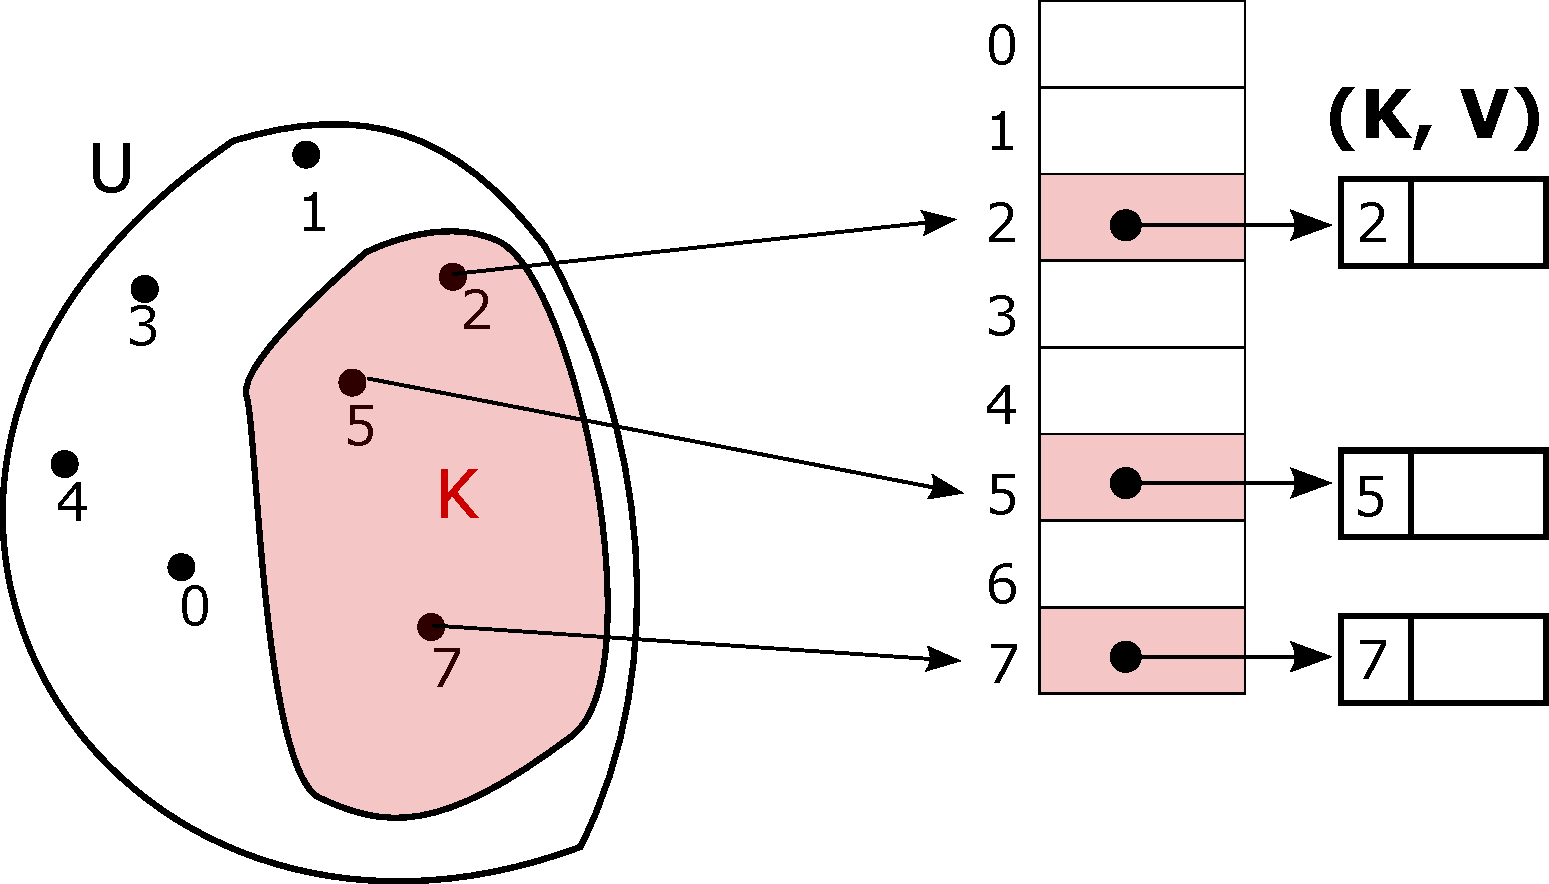
\includegraphics[scale=0.28]{figs/ht_cle_unseq}
\end{figure}
\footnotesize • L'univers des clés possibles est $U$ \\
\footnotesize • $K$ est l'ensemble des clés présentes ($K \subset U$)
\end{frame}






\begin{frame}{Problème 1!}
\pause
Si mon univers est très grand...\\
~\\
\pause

...par rapport au nombre de clés potentielles\\
\pause
~\\
\begin{center}
 \hl{\textbf{Gaspillage de mémoire énorme!}}
 \end{center}
 
 Exemple: Si j'ai des clés bornées entre 0 et 10000 mais a priori jamais plus de 50 valeurs dans ma table: 9950 cases vides.

\end{frame}
\begin{frame}{Problème 2!}
 Et si ma clé est une chaîne de caractères? ou un objet?

\pause
Solution : utilisation d'une \hl{fonction de hachage}
\end{frame}

\subsection{Fonction de hachage}

\begin{frame}{Fonction de hachage}
\begin{block}{Définition}
Une fonction de hachage est une fonction qui transforme une donnée (la clé) en un entier (l'indice dans le tableau).
\end{block}
\hl{Formellement} : h(k) = i \\
\pause
Elle établit une correspondance entre un couple(clé,valeur) et un indice du tableau. Le couple se trouvera à $T[i]$.

\end{frame}

\begin{frame}{Fonction de hachage}

\centering \textbf{Des couples (clé,valeur) stockés dans un tableau}
\begin{block}{}
\begin{figure}
\includegraphics[scale=0.3]{figs/ht_global}
\end{figure}
\end{block}
\end{frame}

\begin{frame}{Fonction de hachage}
\vspace{-1em}
\begin{block}{}
\begin{figure}
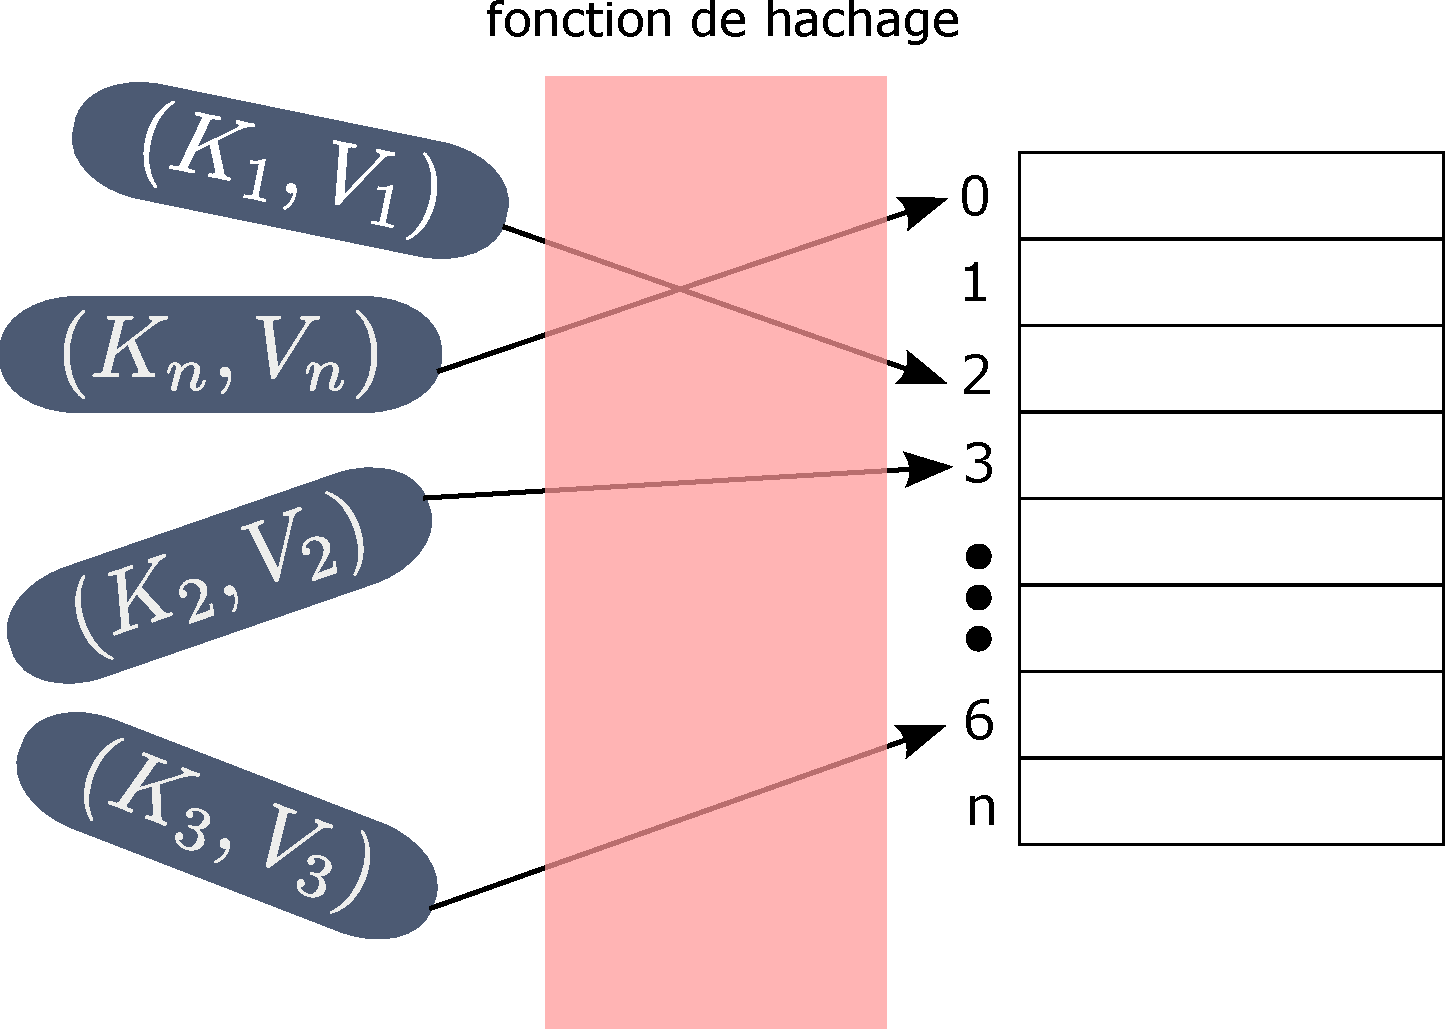
\includegraphics[scale=0.3]{figs/ht_hf}
\end{figure}
\end{block}
\end{frame}

\begin{frame}{Fonction de hachage}
Choix d'une bonne fonction de hachage :
\begin{itemize}
\item Elle doit être cohérente: la même clé produit la même valeur de hachage
\item Elle doit être calculée efficacement 
\item Elle doit distribuer uniformément les clés
\end{itemize}

\end{frame}


\begin{frame}{Adressage direct avec fonction de hachage}
%\begin{block}{}
%...et c'est évidemment pareil si les clés d'origine ne sont pas des entiers.
%\end{block}


\begin{figure}
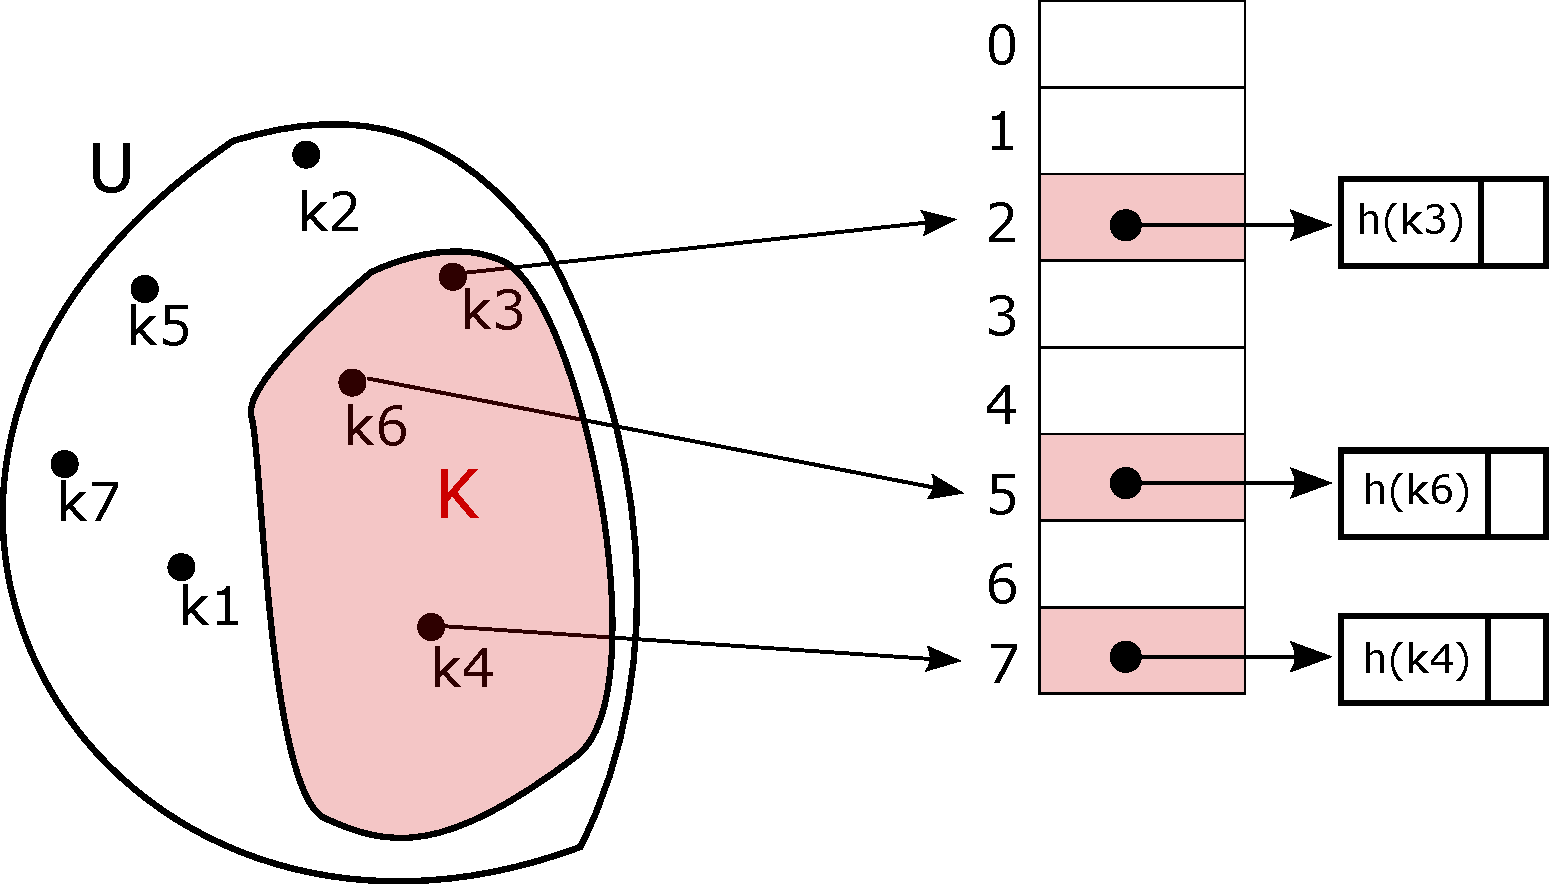
\includegraphics[scale=0.30]{figs/ht_cle_unseq_k}
\end{figure}
Avec
\footnotesize  h(k3) = 2,  h(k4) = 7 et h(k6) = 5.


\end{frame}



\begin{frame}{Exemple de fonction de hachage}{Dictionnaire anglais-français}
Convertir un mot anglais (la clé) en indice:


\begin{itemize}
\item Utiliser la table ascii? \pause \textcolor{red}{\textbf{NON!}}
\pause
\item Coder une lettre par un nombre entre 0 et 27? \pause \textcolor{red}{\textbf{NON!}}
\pause
\item Utiliser une base 27? \pause \textcolor{red}{\textbf{C'est mieux!}}
\end{itemize}
\pause
On a résolu le problème 2, mais pas le 1!
\end{frame}

\begin{frame}{Exemple}{Dictionnaire anglais-français}

\begin{block}{}
On va avoir un tableau de taille faramineuse et beaucoup de cases réservées pour des mots qui n'existent pas!
\end{block}
\begin{table}
    \begin{tabular}{l|lllllll}
 \hl{clé} &   fira   & firb   & firc   & fird   & \textbf{fire}   & firf     \\
   \hl{indice} & 125146 & 125147 & 125148 & 125149 & 125150 & 125151  \\
    \end{tabular}
\end{table}

\end{frame}

\begin{frame}{Hachage}
\begin{itemize}
\item Quelle taille de tableau souhaite-t-on avoir?
\pause
\item Idéalement, une taille proche du nombre d'éléments qu'il y aura effectivement dedans. \pause
\item Comment compresser les valeurs?\pause
\end{itemize}

$\Rightarrow$ \textbf{Utiliser le modulo}
\end{frame}

\begin{frame}{La méthode de la division}
$h(k) =  k \text{ mod } m$ correspond à \textit{la méthode de la division}.
\begin{itemize}
\item  Méthode simple (rapide)
\item Il faut bien choisir la taille $m$ de la table. (nb premier de préférence)
\end{itemize}
$U=2000$ et $m=701$, une moyenne de 3 échecs.\\
\vspace{1.5em}
\textbf{$\triangleright$ Il existe d'autres méthodes...}

\end{frame}




\begin{frame}{Hachage et modulo}

\begin{figure}
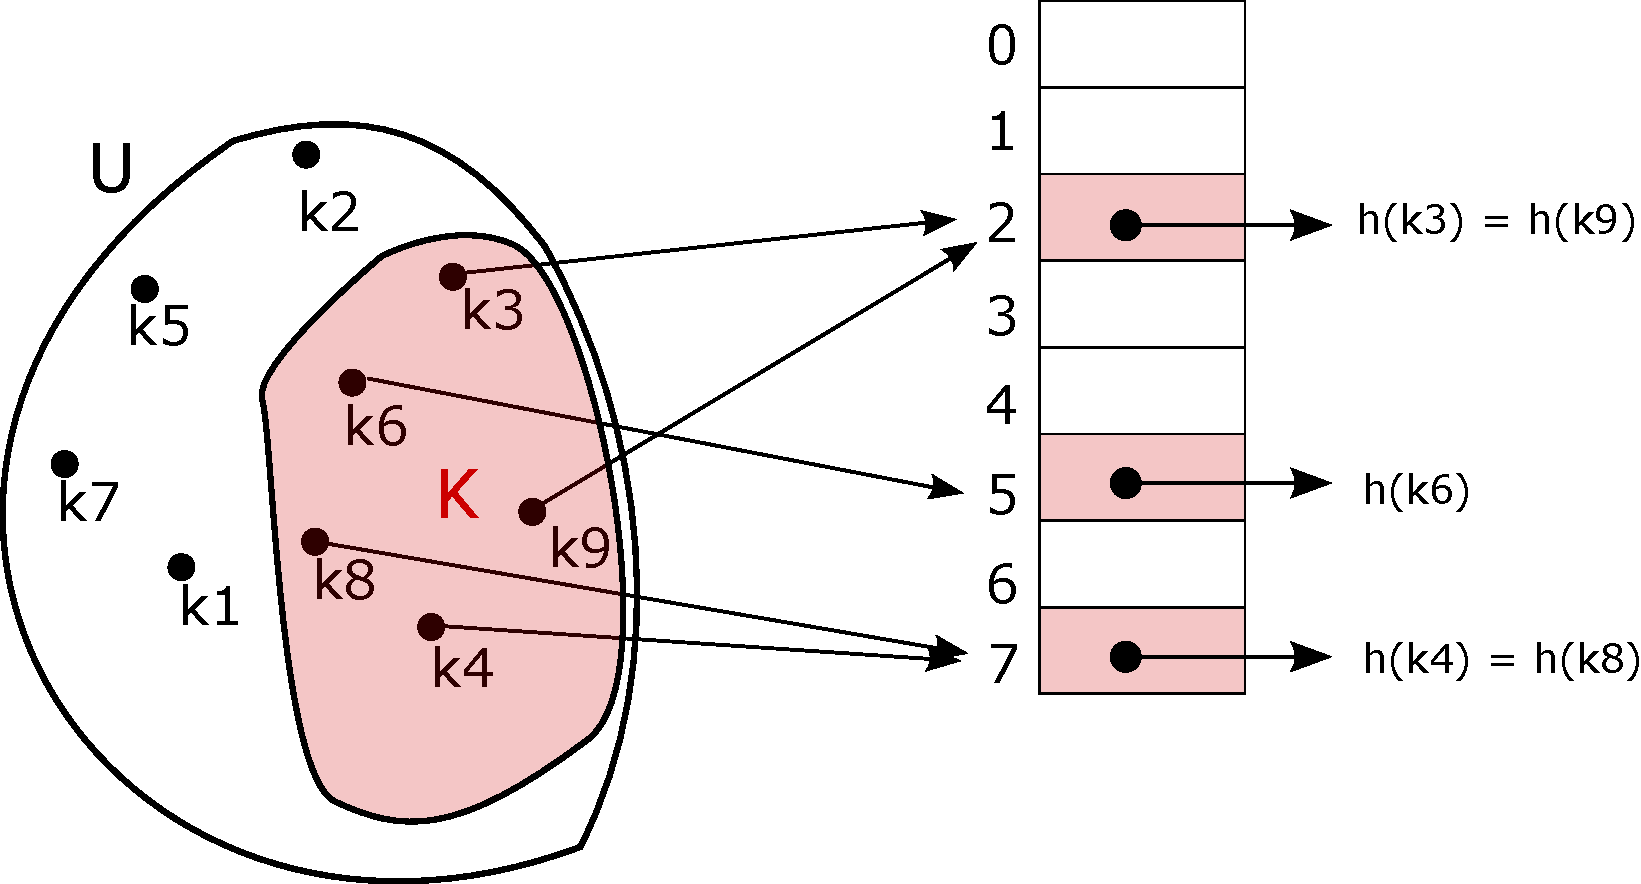
\includegraphics[scale=0.28]{figs/ht_cle_unseq_col}
\end{figure}
\pause
\begin{block}{}
Plusieurs clés correspondent au même indice dans le tableau: c'est une \textbf{collision}.
\end{block}

\end{frame}

\begin{frame}
\tableofcontents
\end{frame}

\section{Gestion des collisions}
\begin{frame}{Collisions}
Pourquoi y a-t-il des collisions?
\begin{itemize}
\item Cas évident : principe des tiroirs
\begin{itemize}
\item Si $n$ chaussettes et $m$ tiroirs et $n>m$\\
$\Rightarrow$ Forcément plus d'une chaussette par tiroir
\end{itemize}
\end{itemize}

\begin{itemize}
\item Si $n < m$, risque de collision tout de même
\begin{itemize}
\item $\Rightarrow$ paradoxe des anniversaires\\
$\Rightarrow$ Dans un groupe de 23 personnes, 50\% de chance qu'il y ait deux personnes avec la même date de naissance.
\end{itemize}
\end{itemize}
\end{frame}

\begin{frame}{Résoudre les collisions}

\begin{itemize}
\item Par adressage ouvert
\item Par chaînage
\end{itemize}

\end{frame}


\subsection{Adressage ouvert}

\begin{frame}
\begin{block}{Principe}
En adressage ouvert, quand un élément ne peut être placé à l'endroit calculé par hachage, on essaie de le placer dans une autre case vide.
\end{block}
\vspace{1em}
Nous allons étudier 3 méthodes:
\begin{itemize}
\item Le sondage linéaire
\item Le sondage quadratique
\item Le hachage double
\end{itemize}
\end{frame}

\begin{frame}{Sondage linéaire}
Soit $i = h(k)$:

\begin{itemize}
\item[1] On accède à $T[i]$ par le retour de la fonction de hachage
\item[2] On regarde si la clé n'est pas dans la case $h(k)+1$:
\item[3] \textbf{En cas d'insertion} : on ajoute dans la première case vide trouvée\\
\textbf{En cas de recherche} : Tant qu'on a pas trouvé la valeur on répète 2.\\
Si on trouve une case vide, la donnée n'existe pas.
\end{itemize}
On regarde aux indices $h(k)+2, h(k)+3, h(k)+4...$\\
\vspace{1em}
\pause \Frowny Problème de clustering (pire si la table est trop remplie).
\end{frame}

\begin{frame}
\begin{figure}
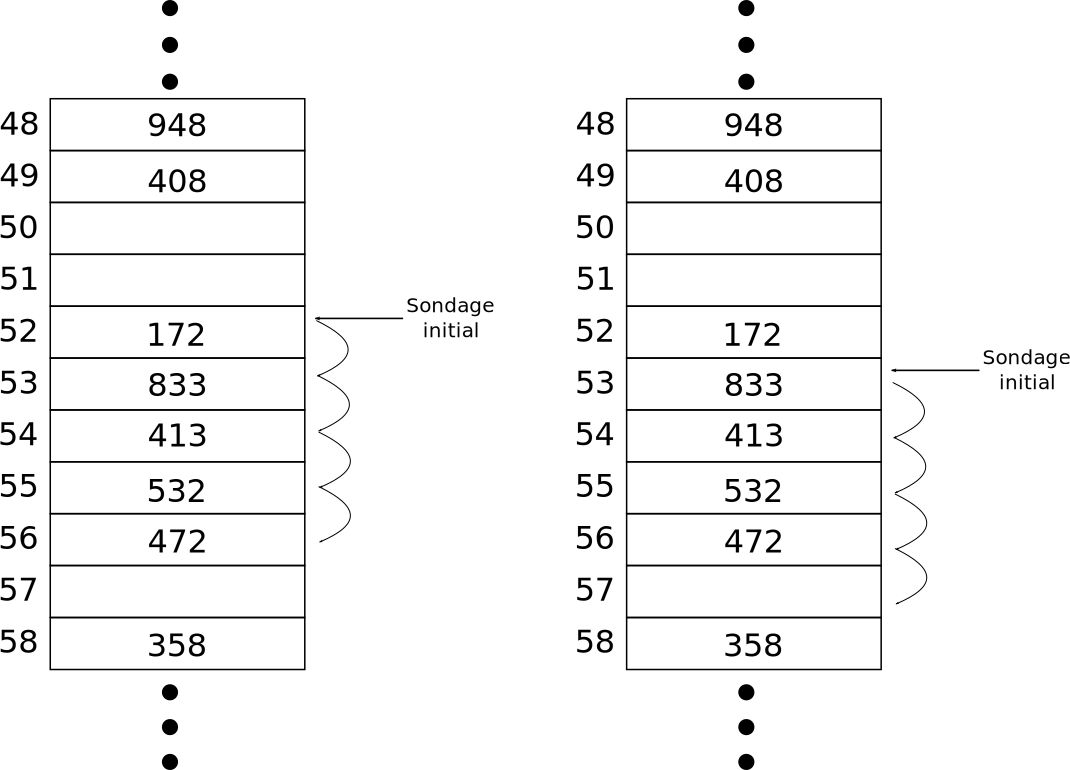
\includegraphics[scale=0.3]{figs/ht_linear}
\end{figure}
\hspace{-1em}a)Recherche réussie de 472  \hspace{1em}  b)Recherche infructueuse de 893
\end{frame}

\begin{frame}{Sondage quadratique}

\begin{itemize}
\item On ne regarde plus juste à la case suivante.
\item On applique une fonction quadratique à pour passer d'une case à l'autre
\end{itemize}

On regarde aux indices $h+1^2, h+2^2, h+3^2, h+4^2,...  h+i^2 ...$ ou plus
généralement aux indices $h(k) + \alpha i + \beta i^2$.

\pause \Frowny Problème de clustering secondaire.

\end{frame}

\begin{frame}
\begin{figure}
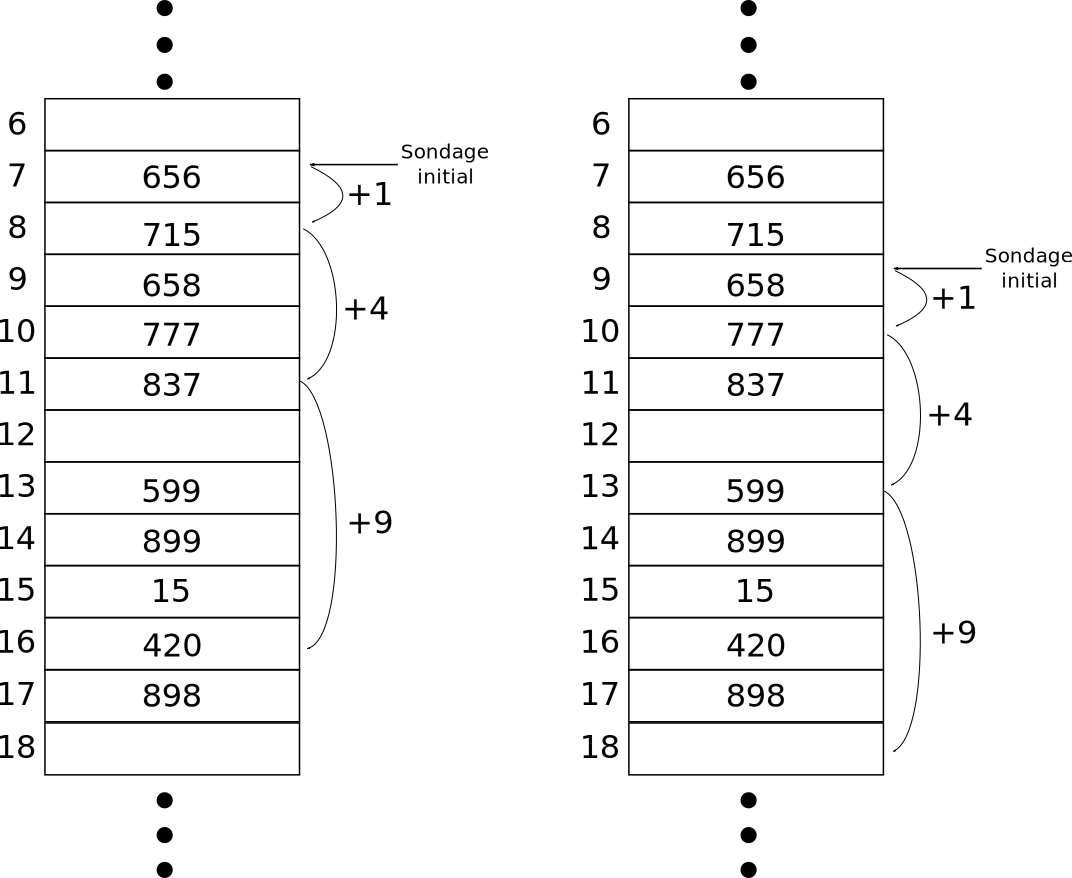
\includegraphics[scale=0.28]{figs/ht_quad}
\end{figure}
\hspace{-1em}a)Recherche réussie de 420  \hspace{1em}  b)Recherche infructueuse de 480
\end{frame}


\begin{frame}
Pour que le sondage soit efficace:
\begin{itemize}
\item Le \hl{facteur de charge} doit être limité (pas plus 2/3)\\
$facteur de charge = nbElements/tailleTable$
\item On ne peut avoir plus d’éléments que de cases du tableau
\end{itemize}
\end{frame}



\begin{frame}{Double Hachage}
Les sondages linéaire et quadratique posent des problèmes de clustering car on suit toujours la même séquence.\pause \\
\vspace{1em}
Une solution : \hl{Le double hachage}

\begin{block}{Principe}
On va utiliser une seconde fonction de hachage sur les deux clés qui va déterminer un pas (probablement) différent.
\end{block}

\end{frame}

\subsection{Chaînage séparé}
\begin{frame}
Jusque qu'ici, au maximum autant d'objets que la taille de la table.
\begin{block}{Principe}
On va ranger tous les couples dont les clés ont la même valeur de hachage dans une liste chaînée 
\end{block}
\end{frame}
\begin{frame}
\begin{figure}
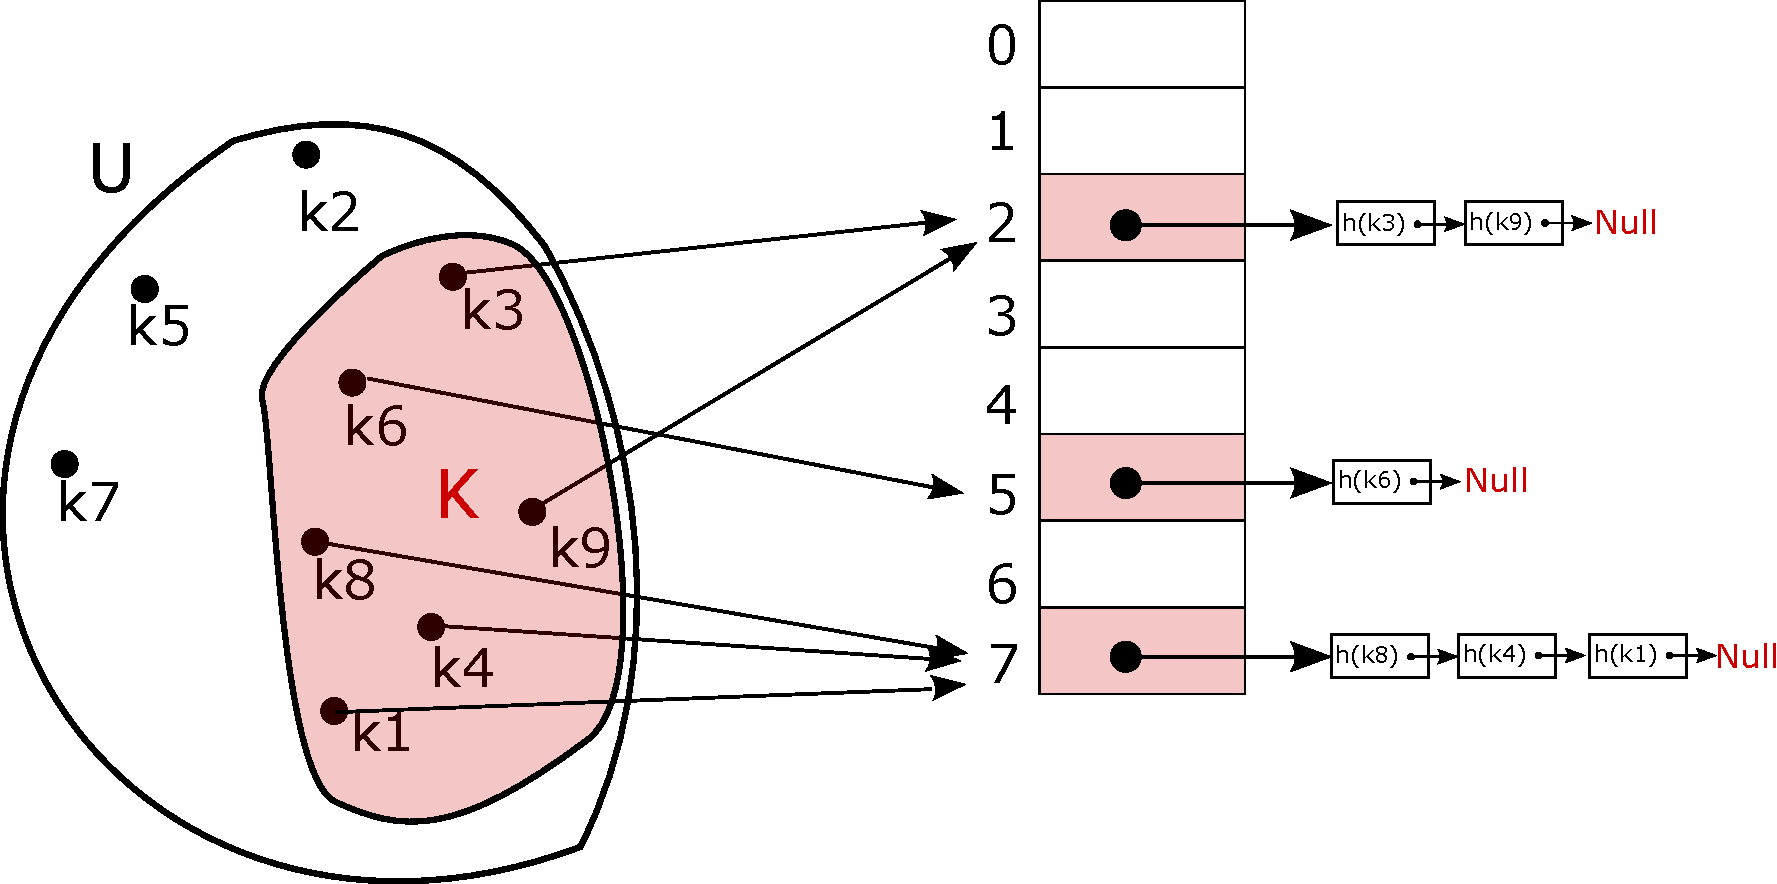
\includegraphics[scale=0.35]{figs/ht_chaining}
\end{figure}
\end{frame}

\begin{frame}
\tableofcontents
\end{frame}

\subsection{HashMap}

\begin{frame}[fragile]
Nous utiliserons le plus souvent la classe \texttt{HashMap} de l'interface \texttt{Map}.\\
Exemple d'utilisation:

\begin{lstlisting}[language=Java]
 public static void main(String[] args) {
     Map <String,Integer> iMap 
     = new HashMap<String,Integer>();
     iMap.put("one", new Integer(1));
     iMap.put("two",new Integer(3));
     iMap.put(null, new Integer(45));
     iMap.put(null, new Integer(32));
		
     Integer i = iMap.get("three"); //Retourne null
     Integer j = iMap.get("one"); // j = 1
     System.out.println(iMap.get(null)); //affiche 32
 }
\end{lstlisting}

\end{frame}

\section{Les tables de hachage en java}

\subsection{equals() et hashcode()}

\begin{frame}{Egalité d'objets}
\begin{block}{}
L'opérateur $==$ compare l'égalité des références des objets et la méthode \texttt{equals()} leur égalité tout court.
\end{block}

\begin{itemize}
\item Mais par défaut \texttt{equals()} se base sur les références.
\item Il faut donc la \hl{redéfinir}!
\item Sinon deux instances aux mêmes propriétés seront considérées comme différentes!
\end{itemize}
\end{frame}

\begin{frame}{La méthode \texttt{hashcode}}
En Java, la valeur de la fonction de hachage est implicite à chaque objet:
\begin{itemize}
\item La méthode \texttt{hashcode} de \texttt{Object} renvoie la valeur de hachage.
\item Par défaut, elle fait référence à l'emplacement mémoire comme \texttt{equals}.
\end{itemize}
\begin{block}{}
Si a.equals(b) => a.hashcode() == b.hashcode\\
Mais la réciproque est fausse!
\end{block}
\pause
Il est donc important de redéfinir conjointement ces méthodes!
\end{frame}



\section{Set}

\begin{frame}
\tableofcontents
\end{frame}

\begin{frame}{Set}
Les Set sont des ensembles d'objets:

\begin{itemize}
\item Uniquement des objets (pas de couple(clé,valeur))
\item Pas de doublon
\item Pas d'ordre
\item Relatif à la notion d'ensemble en mathématiques.
\end{itemize}

En Java, l'implémentation de l'interface \texttt{Set} \texttt{HashSet} est basée sur l'utilisation d'une \texttt{HashMap}.

\end{frame}

\begin{frame}[fragile]

\begin{lstlisting}[language=Java]

HashSet<String> etatsSet = new HashSet<String>();
etatsSet.add ("FR");
etatsSet.add ("AG");
etatsSet.add ("CU");
 
if(etatsSet.contains("MX")) {
  System.out.println("Deja trouve");
}else{
  etatsSet.add("MX");
}


\end{lstlisting}
\end{frame}


\begin{frame}{Entry(K,V) de Map}
\begin{itemize}
\item La méthode \texttt{Set< Map.Entry<K,V> > entrySet()} retourne un Set de Map.Entry<K,V> qui correspond à un couple (clé,valeur).
\item Le \texttt{Set} retourné correspond à une vue sur la \texttt{Map} à l'instant $t$.
\item On peut appeler les méthodes \texttt{getKey()} and \texttt{getValue()} pour accéder respectivement aux clés et aux valeurs.
\end{itemize}

\end{frame}

\begin{frame}[fragile]
\begin{lstlisting}[language=Java]
 public static void main(String[] args) {
     Map <String,Integer> iMap = 
     new HashMap<String,Integer>();
     iMap.put("one", new Integer(1));
     iMap.put("two",new Integer(3));
     iMap.put(null, new Integer(45));
     iMap.put(null, new Integer(32));
     
     Set<Entry<String, Integer>>  set = iMap.entrySet();
     System.out.println("valeur d'un set: " + set);
     //valeur d'un set: [null=32, two=3, one=1]
 }
\end{lstlisting}

\end{frame}


\begin{frame}{Au delà du cours : Empreinte MD5}
\emph{Empreinte MD5} : fonction de hachage cryptographique calculée sur un fichier.\\
$\Rightarrow$ Permet de vérifier l'intégrité d'un fichier.\\
Scénario exemple:

\begin{itemize}
\item Je télécharge une version d'ubuntu
\item Je veux être certain que mon fichier téléchargé n'est pas corrompu ou vérolé
\item Je récupère l'empreinte MD5 sur le site de source officielle
\item Je calcule cette empreinte avec un utilitaire comme \texttt{md5sum}
\item Je compare cette empreinte avec l'officielle
\item Si elles correspondent, je peux faire confiance à mon fichier.
\end{itemize}

\end{frame}



\begin{frame}
Dans ce cours, nous avons vu:
\begin{itemize}
\item Le fonctionnement des tables de hachages,
\item La résolution des collisions,
\item Comment on les utilise en pratique (c'est simple)!
\end{itemize}
\end{frame}


\end{document}

